\documentclass{beamer}

\title{Atreus, i3, and Vim}
\subtitle{An overview of mechanical keyboards and optimizing workflow}
\author{Loren Rogers}
\date{April 6, 2016}
\titlegraphic{ 
\includegraphics[scale=0.3]{images/vim-logo} }

\begin{document}

\maketitle

\begin{frame}
  \frametitle{Hi, I'm Loren}
  \begin{itemize}
    \item I'm a UX designer at EMC
    \item Twitter: @lorentrogers
    \item Presentation built with \LaTeX, available on Github.
  \end{itemize}
\end{frame}

\begin{frame}
  \frametitle{We Know Vim is Awesome}
  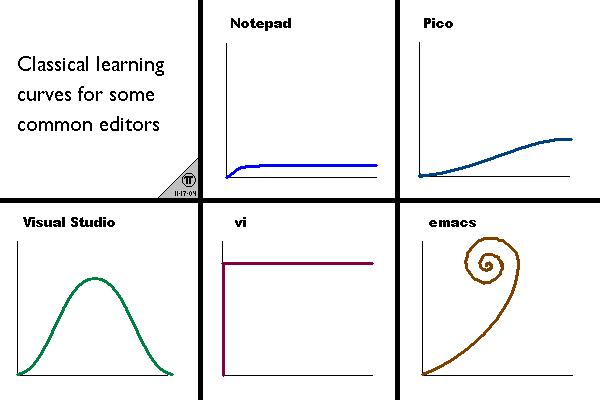
\includegraphics[scale=0.5]{images/curves}
  \begin{itemize}
    \item But it's an investment...
  \end{itemize}
\end{frame}

\begin{frame}
  \frametitle{The End-Goal}
  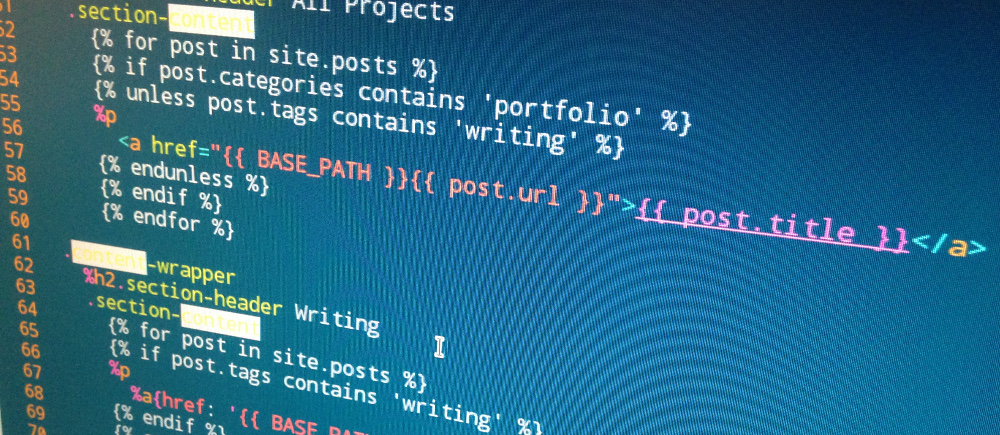
\includegraphics[scale=0.2]{images/vim}

  \begin{itemize}
    \item Long-term investment
    \item Small number of quality tools
    \item Looking outside of Vim
    \item Ecosystem
    \item How do you pick tools?
  \end{itemize}
\end{frame}

\begin{frame}
  \frametitle{Design Perspective}

  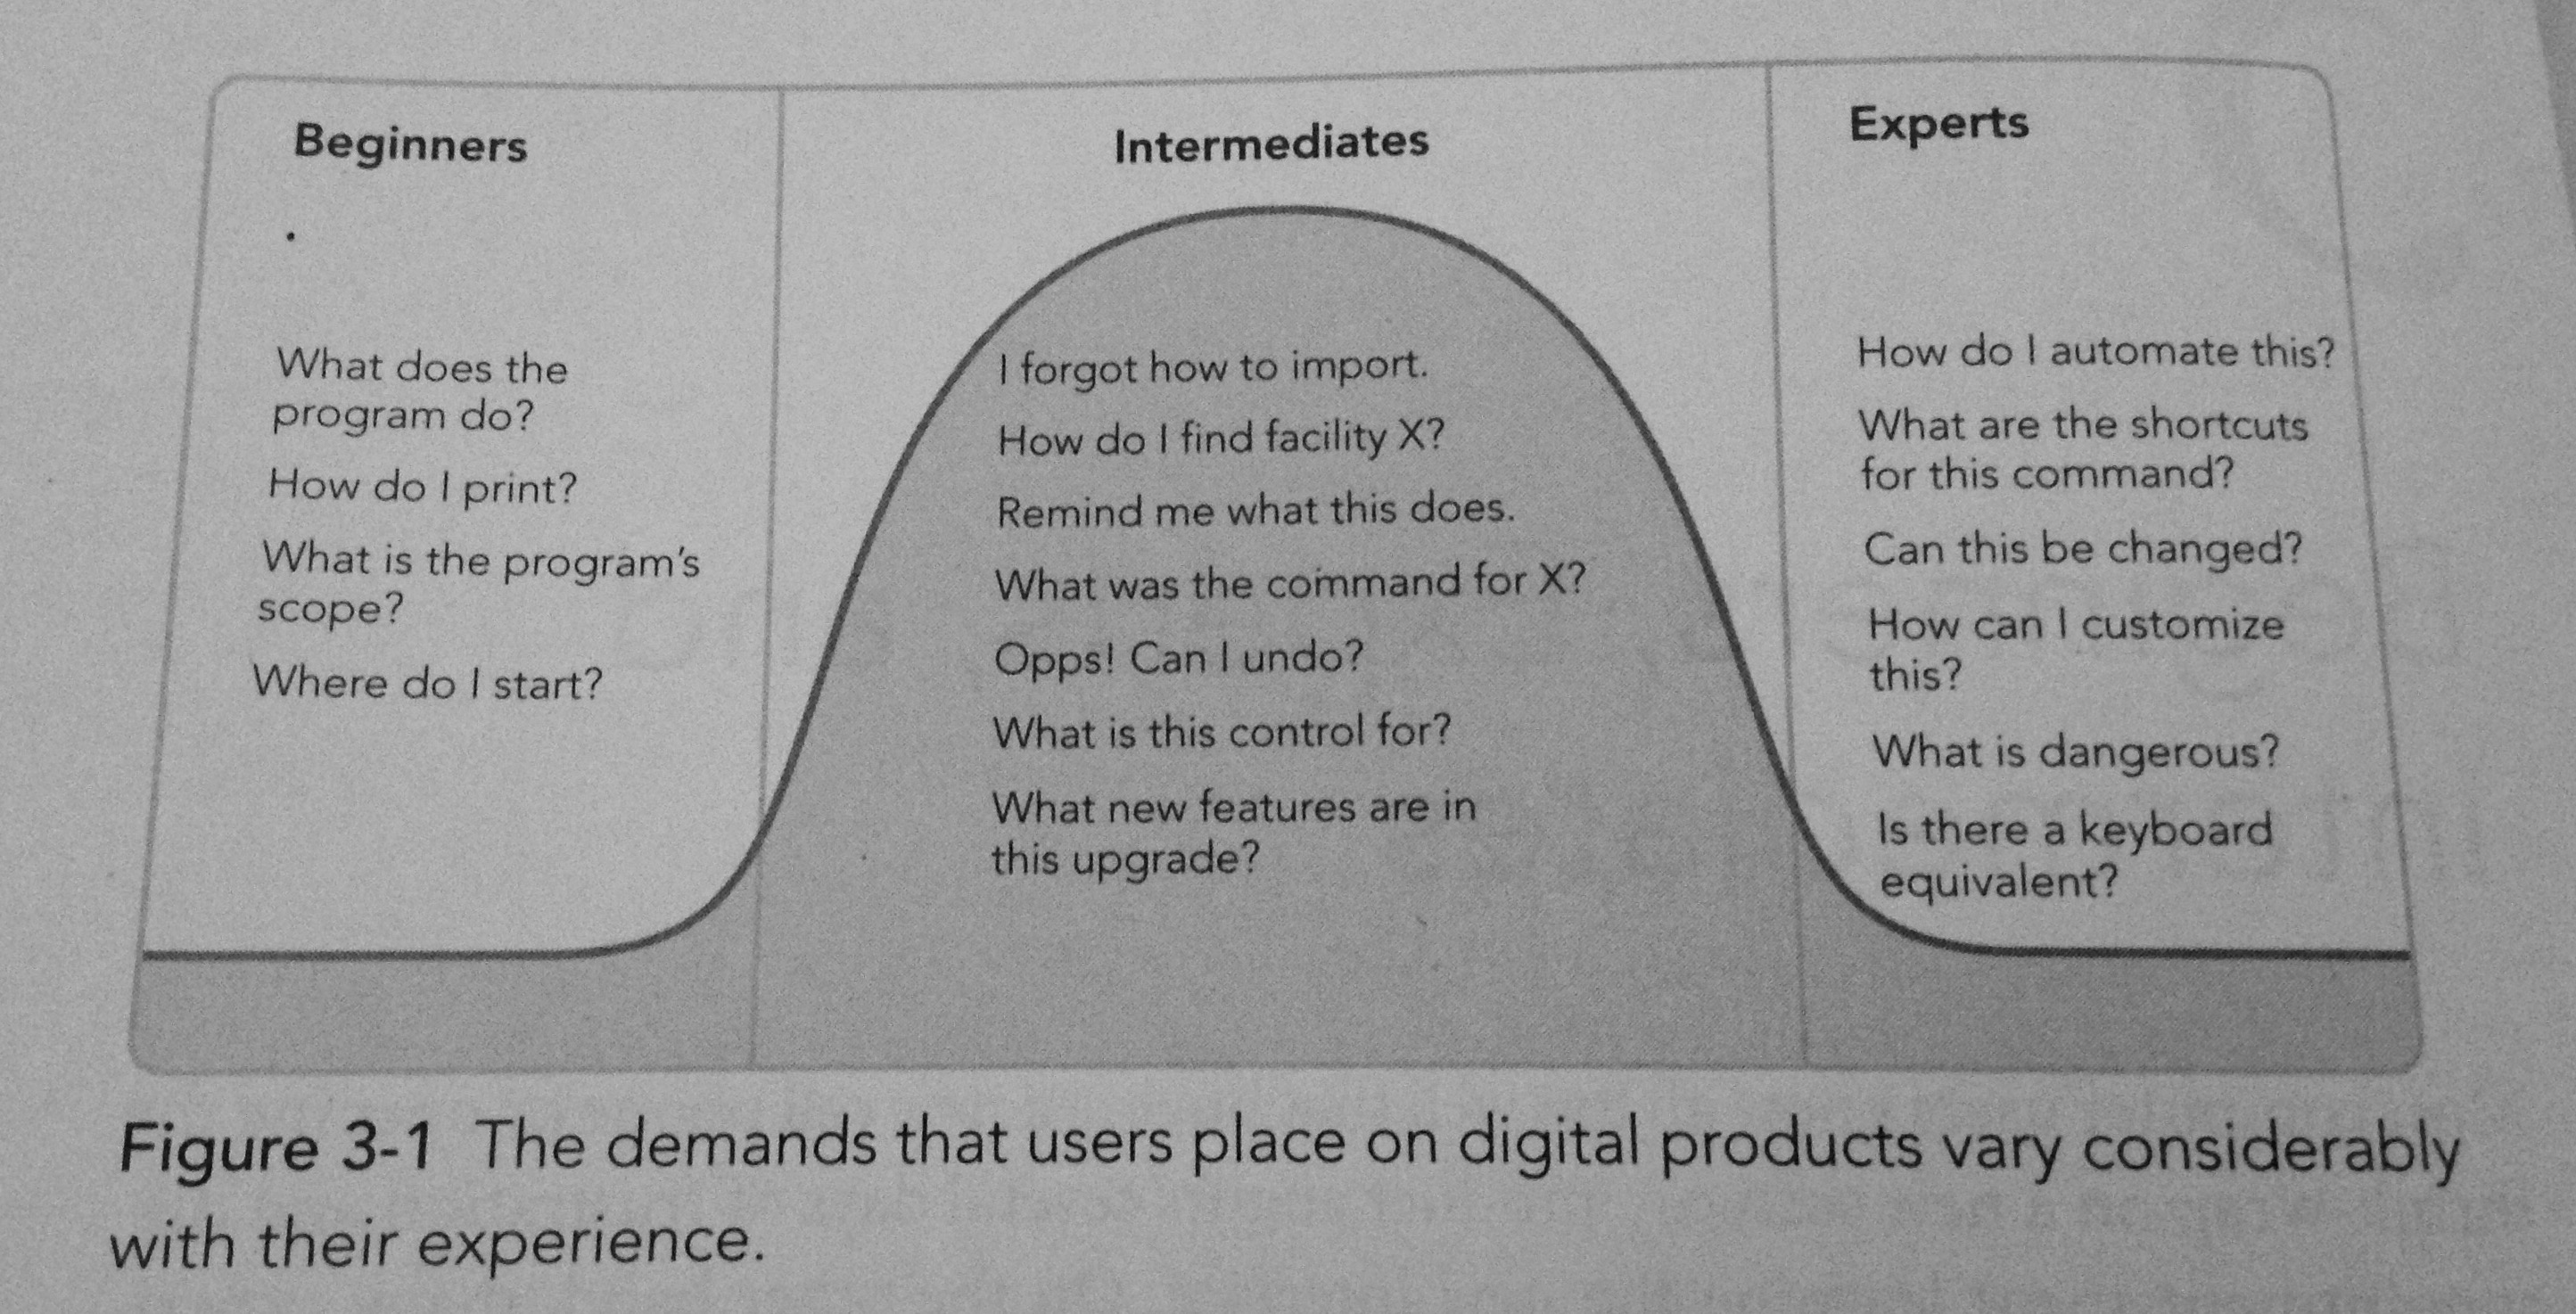
\includegraphics[scale=0.1]{images/about-face-diagram}

  \begin{itemize}
    \item We're going for expert: intuition be damned.
    \item Use the same patterns as much as possible across platforms.
    \item Keep information in the mind, rather than in the world.
  \end{itemize}
\end{frame}

\begin{frame}
  \frametitle{Window Manager \& Keyboard}
  Things we'll look at today:
  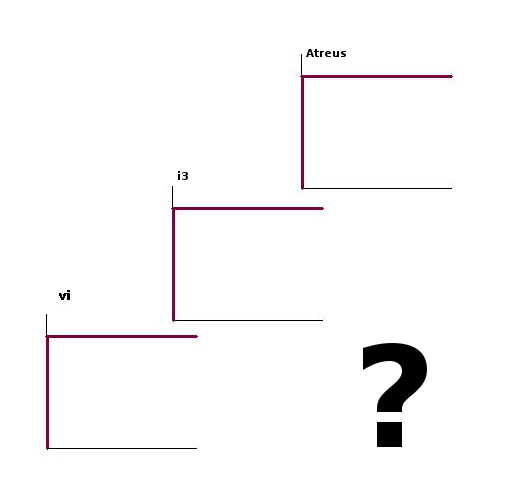
\includegraphics[scale=0.5]{images/ladder}
\end{frame}

\begin{frame}
  \frametitle{i3wm}
  \begin{itemize}
    \item Tiling window manager
    \item Open source
    \item Focus on configuration, simplicity, speed
    \item Awesome.
  \end{itemize}
  
\includegraphics[scale=0.3]{images/i3wm}
\end{frame}

\begin{frame}
  \frametitle{i3wm Configuration}
  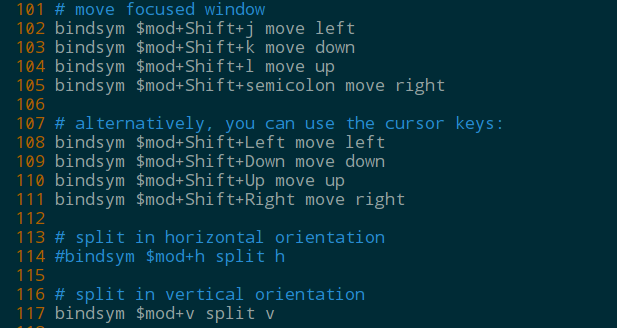
\includegraphics[scale=0.5]{images/i3-config-example}
\end{frame}

\begin{frame}
  \frametitle{i3wm Configuration}
  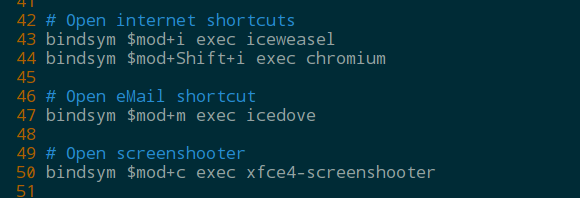
\includegraphics[scale=0.5]{images/i3-internet-config}
\end{frame}

\begin{frame}
  \frametitle{i3wm Configuration}
  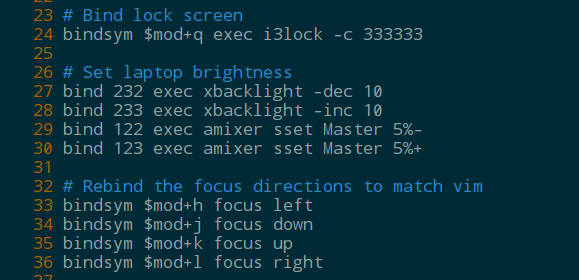
\includegraphics[scale=0.5]{images/i3-lock-and-move-config}
\end{frame}

\begin{frame}
  \frametitle{Demonstration}
  (Demo time!)

  \begin{itemize}
    \item Opening browsers, terminals
    \item Moving around monitors
    \item Quick tasks: e.g. JekyllJournal
  \end{itemize}
\end{frame}

\begin{frame}
  \frametitle{Why i3 Rules}
  \begin{itemize}
    \item Very quick access to common functions (new term, browser, email)
    \item Open apps by name, not icon
    \item Really easy to customize / integrate w/ vim, tmux, keyboard
    \item Many desktops help keep you organized
  \end{itemize}
\end{frame}

\begin{frame}
  \frametitle{Keyboard}
  Your setup matters!
  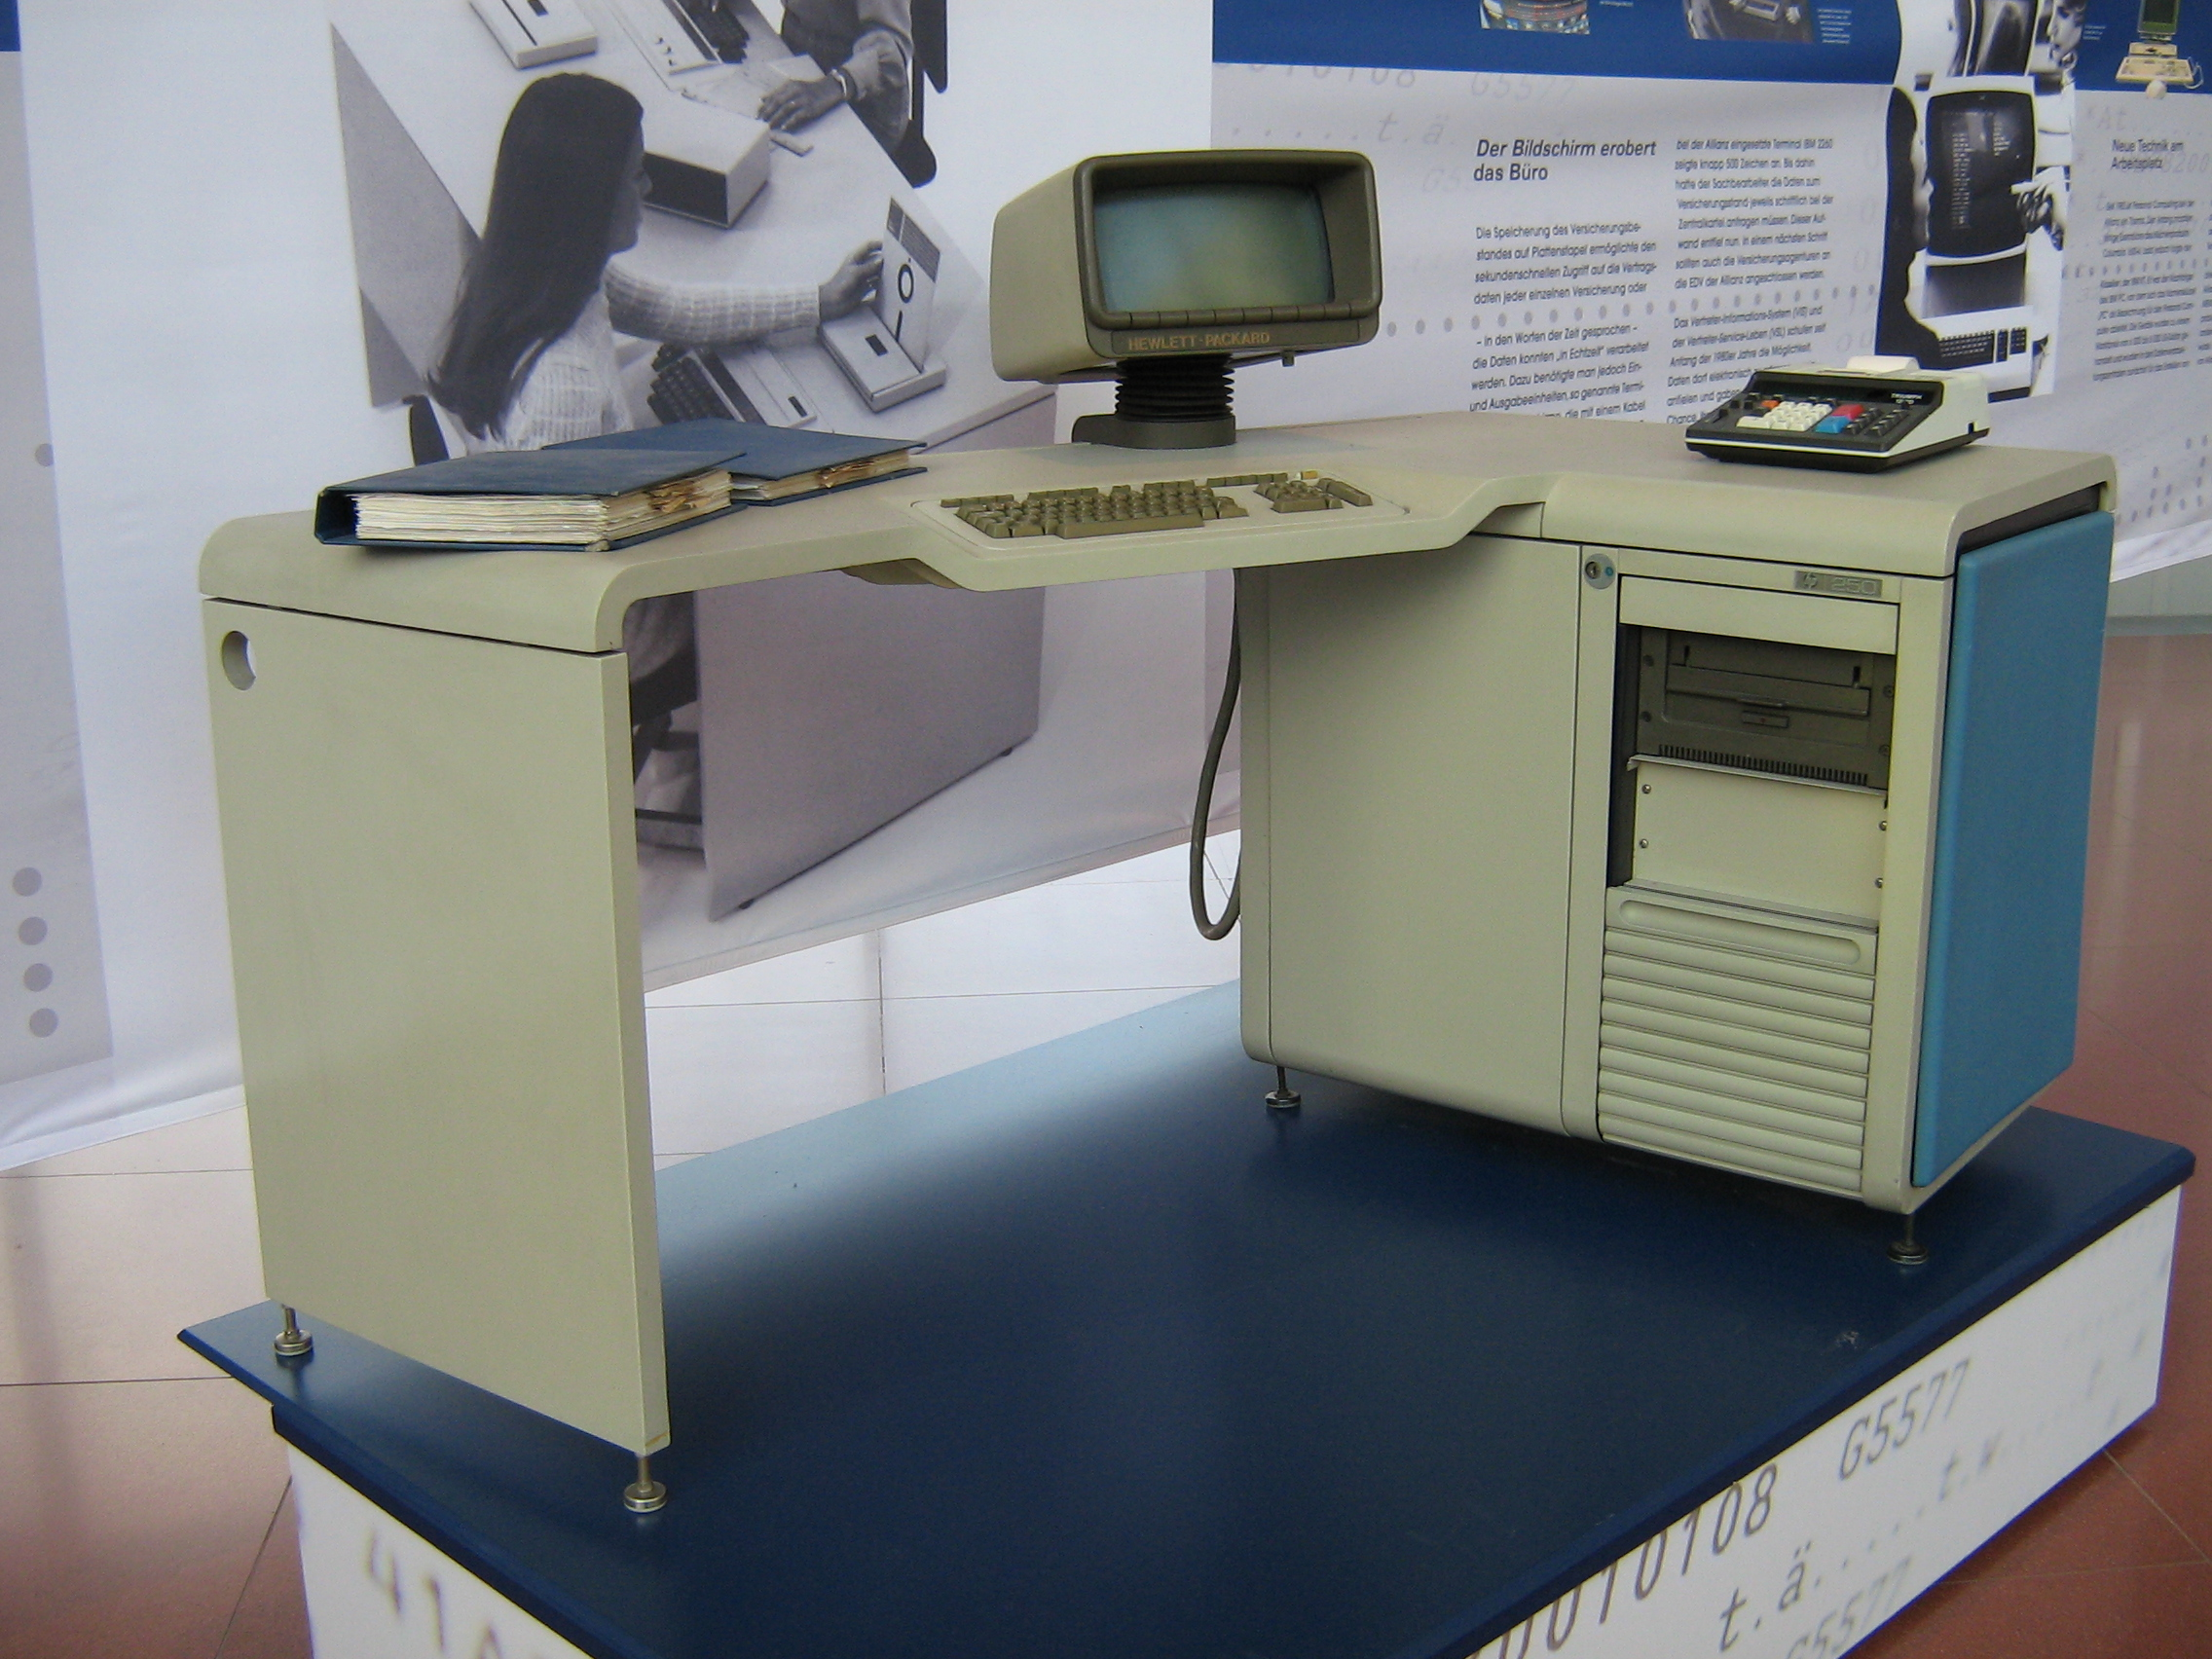
\includegraphics[scale=0.1]{images/awesome-system}
\end{frame}

\begin{frame}
  \frametitle{Mechanical Keyboards}
  Why should I care?
  \begin{itemize}
    \item Comfort: mechanical vs dome membrane
    \item Speed \& combinations
    \item Layout ergonomics
  \end{itemize}
\end{frame}

\begin{frame}
  \frametitle{Speed and Options}
  On many keyboards, these are all equivalent keystrokes!
  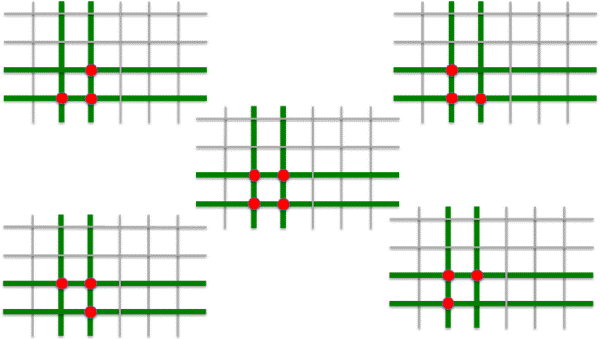
\includegraphics[scale=0.7]{images/multi-press}
\end{frame}

\begin{frame}
  \frametitle{Actuation}
  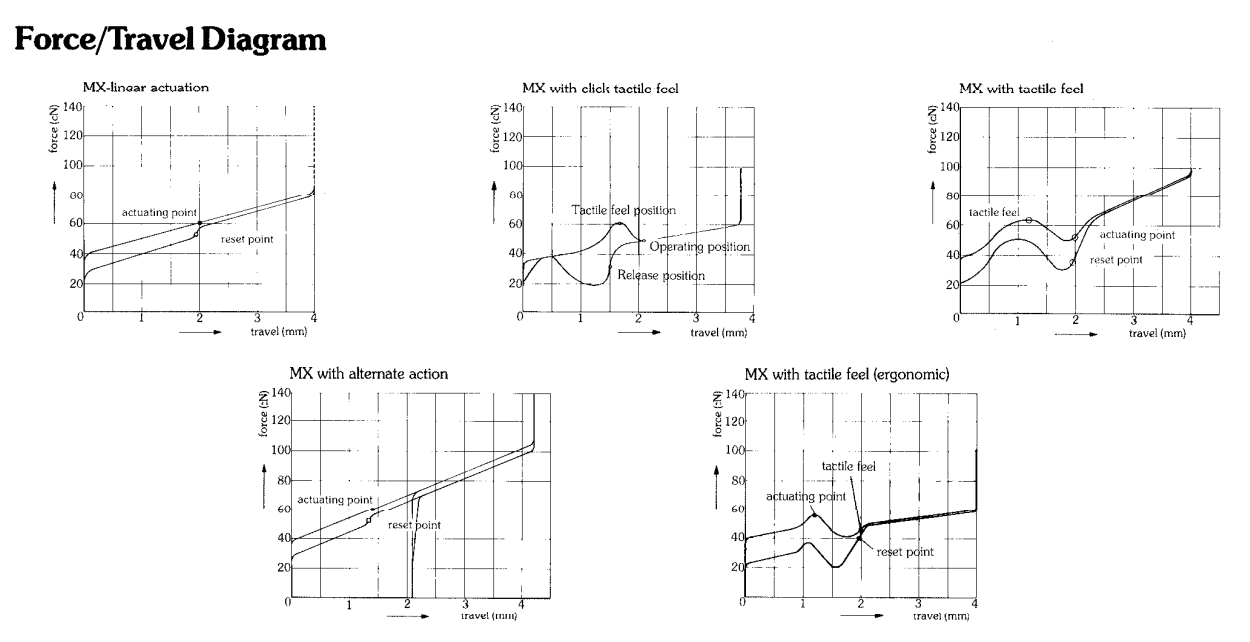
\includegraphics[scale=0.25]{images/force-travel-diagram}
\end{frame}

% layouts

\begin{frame}
  \frametitle{Layouts}
  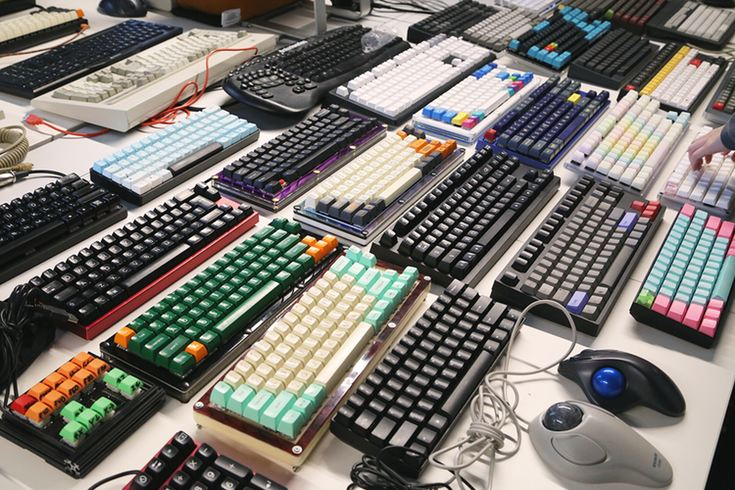
\includegraphics[scale=0.4]{images/options}
\end{frame}

\begin{frame}
  \frametitle{Layouts}
  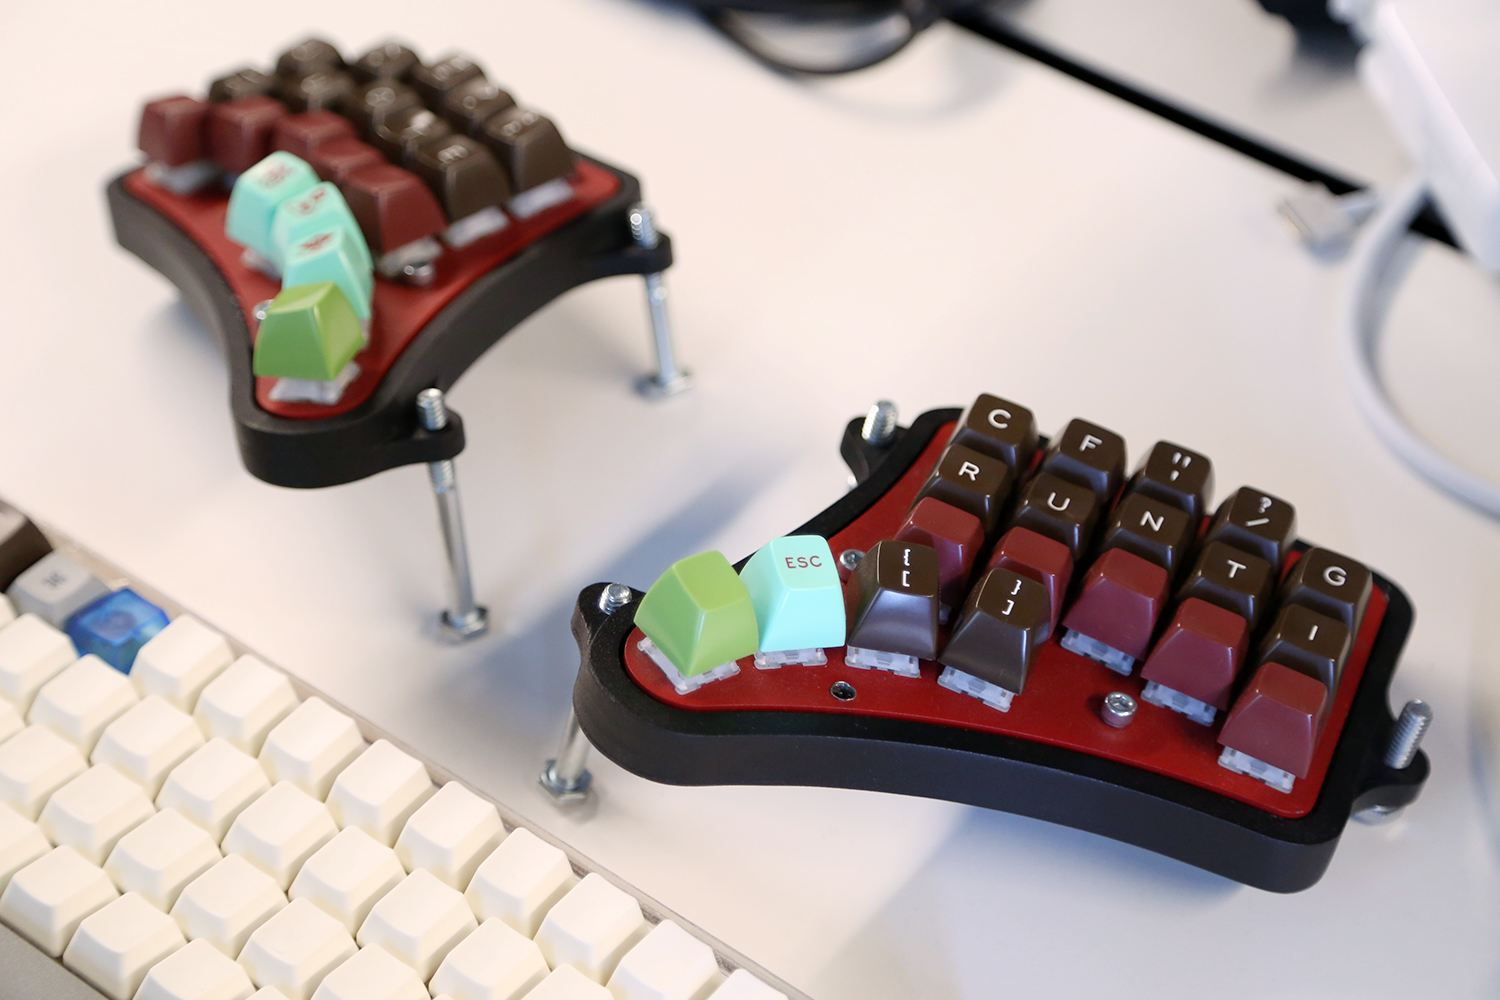
\includegraphics[scale=0.2]{images/custom-layout}

  \tiny https://www.massdrop.com/article/kiibohd-16-mech-meetup-md
\end{frame}

% keymaps

\begin{frame}
  \frametitle{Keymaps}
  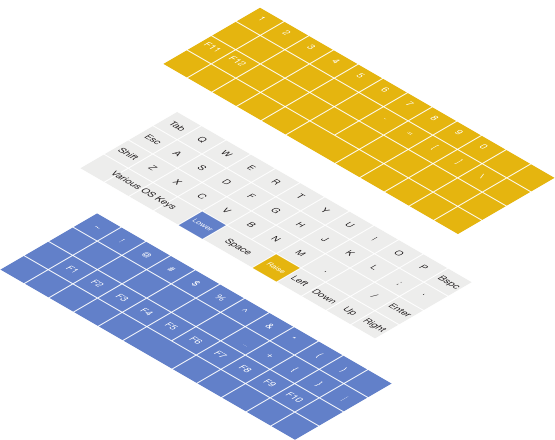
\includegraphics[scale=0.5]{images/planck}

  Planck
\end{frame}

\begin{frame}
  \frametitle{Keymaps}
  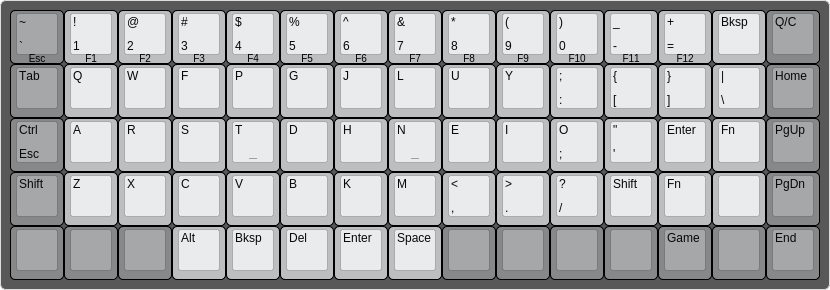
\includegraphics[scale=0.35]{images/atomic-layout}

  Atomic
\end{frame}

\begin{frame}
  \frametitle{Keymaps}
  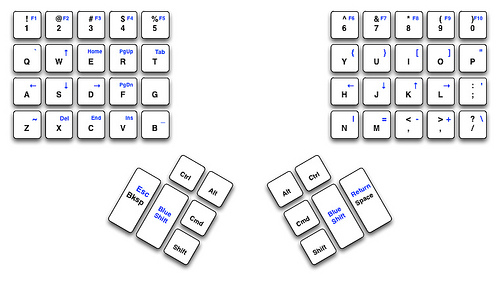
\includegraphics[scale=0.5]{images/ergodox-layout}

  Ergodox
\end{frame}








\begin{frame}
  \frametitle{Atreus}
  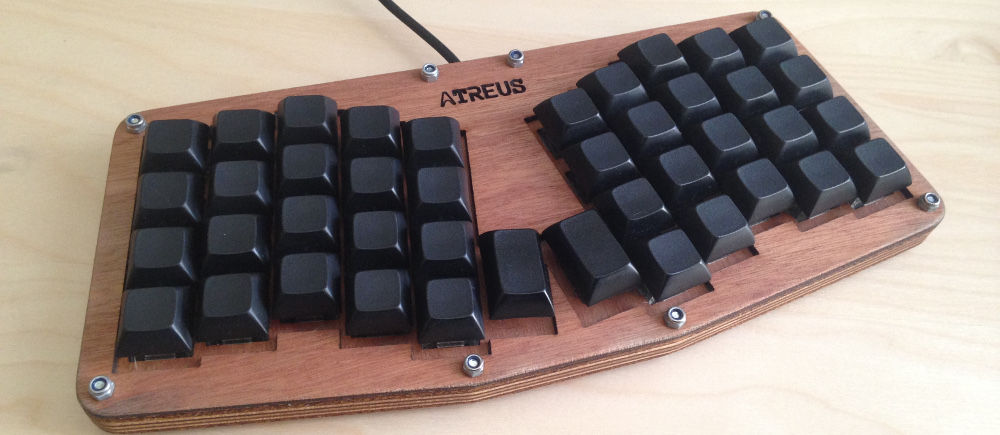
\includegraphics[scale=0.3]{images/atreus}
\end{frame}

\begin{frame}
  \frametitle{Atreus}
  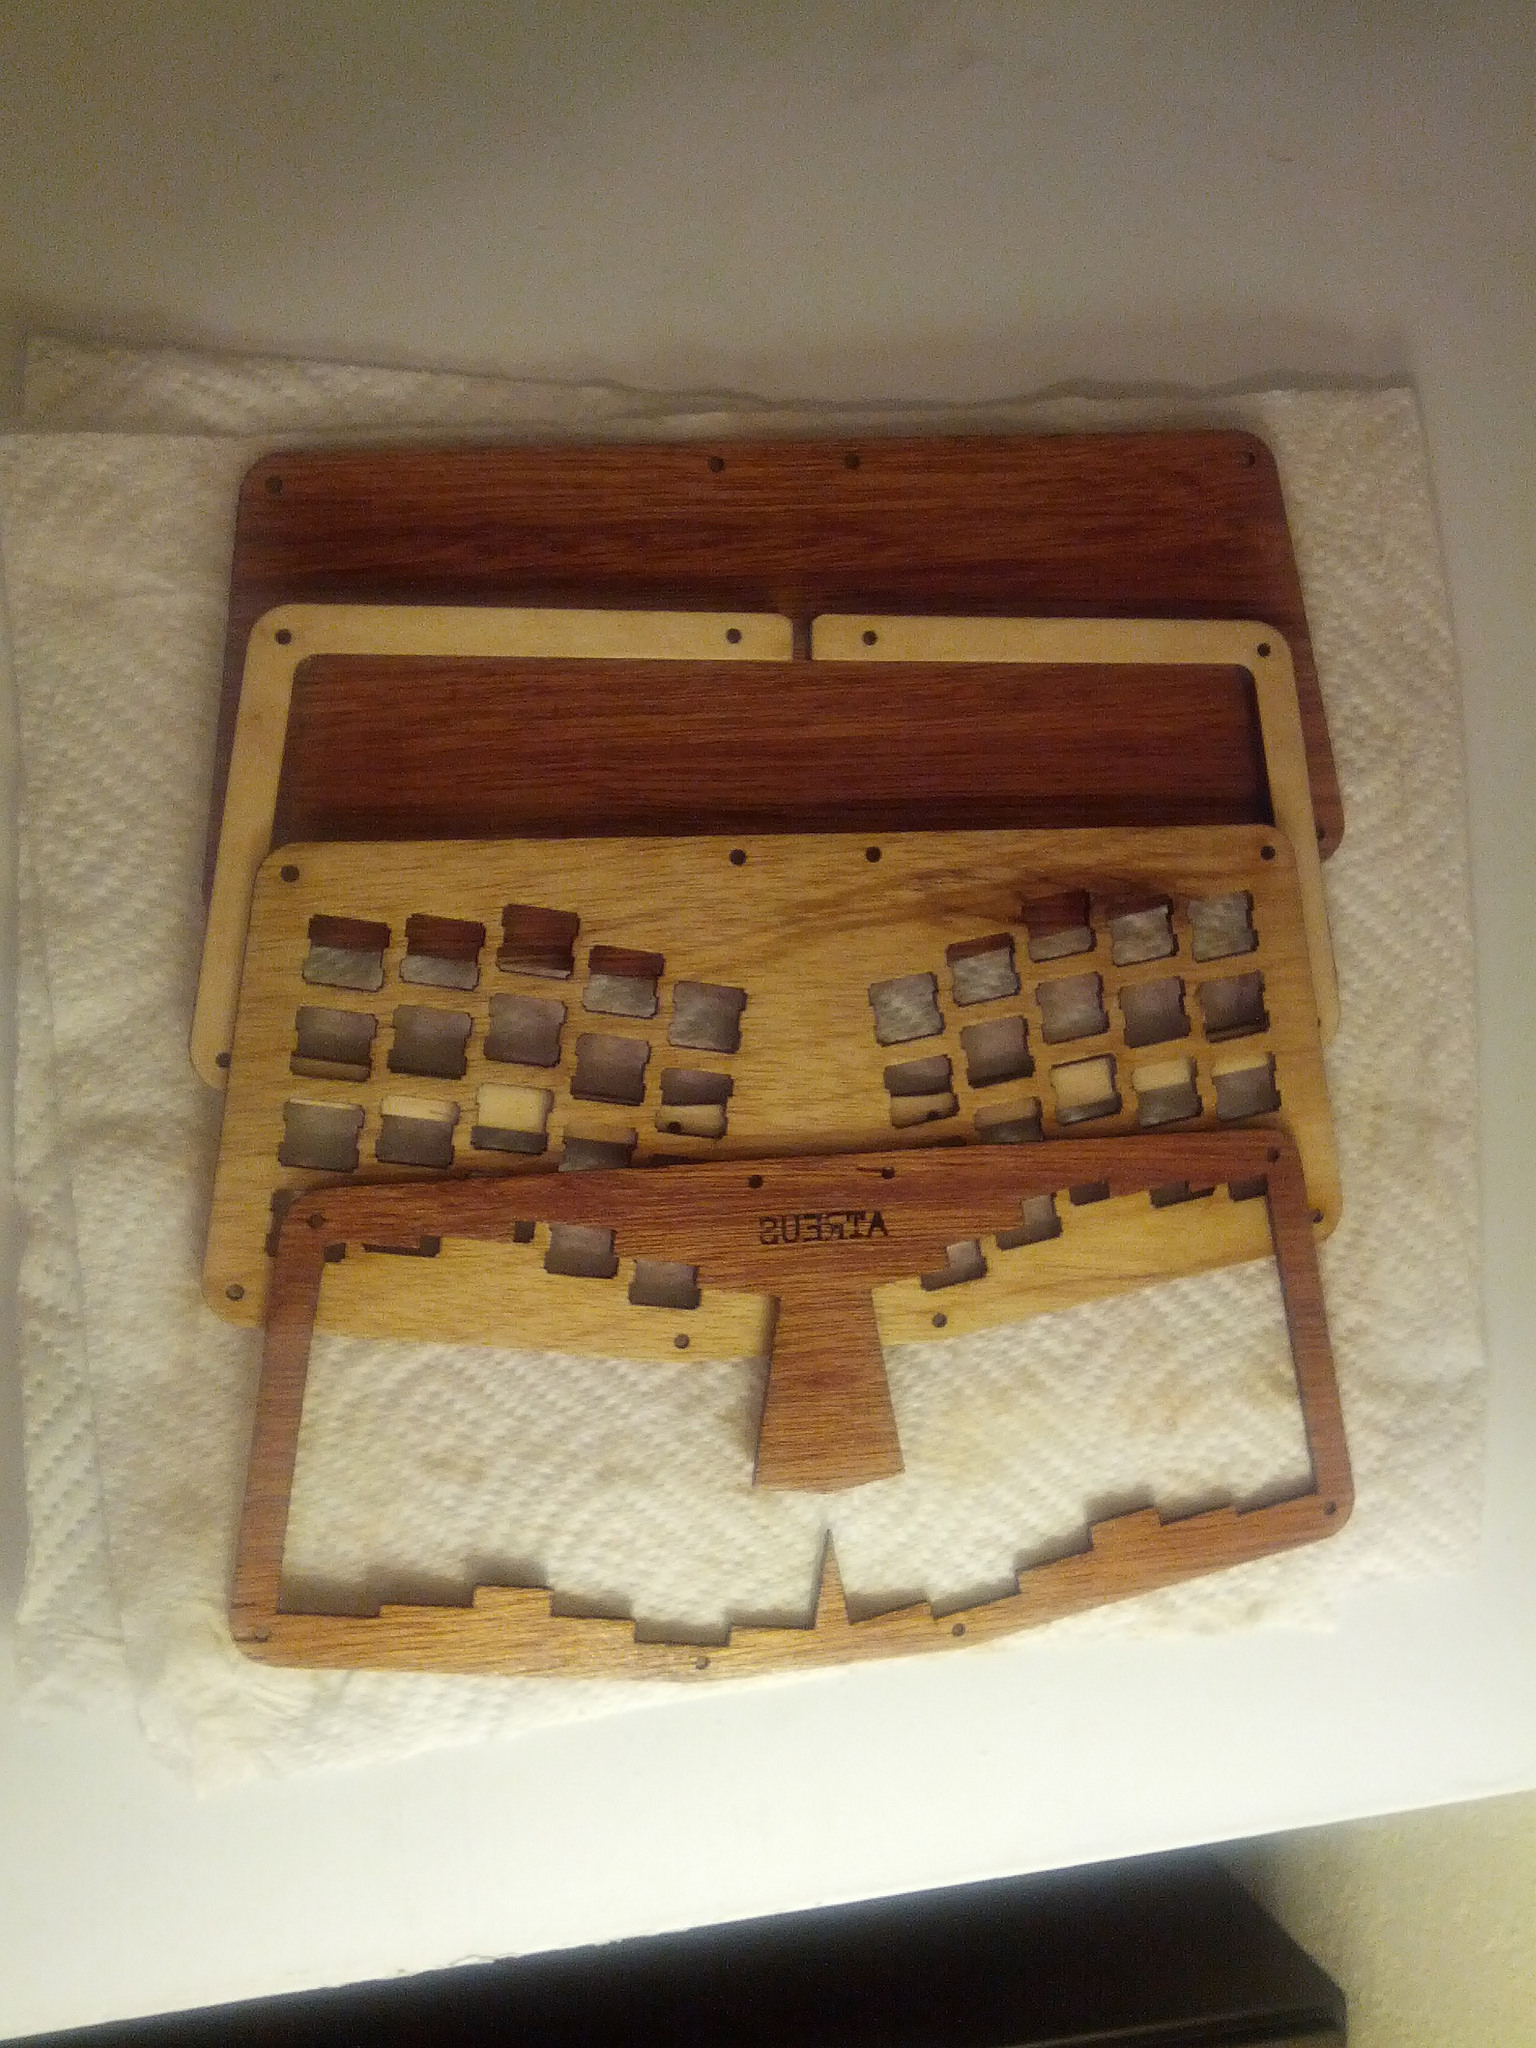
\includegraphics[scale=0.1]{images/atreus-body}
\end{frame}

\begin{frame}
  \frametitle{Atreus}
  Why I chose this specific keyboard:
  \begin{itemize}
    \item Open source
    \item Portable
    \item Customizable
    \item Column layout (also called ortholinear)
    \item Layered firmware
  \end{itemize}
\end{frame}




\begin{frame}
  \frametitle{Atreus: Layer 0}
  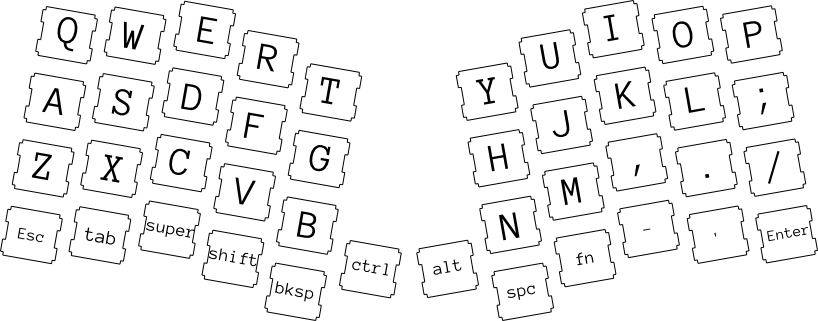
\includegraphics[scale=0.45]{images/atreus-layer-1}
\end{frame}

\begin{frame}
  \frametitle{Atreus: Layer 1}
  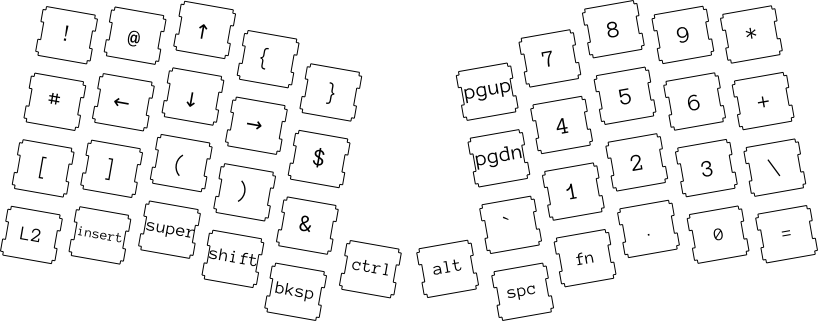
\includegraphics[scale=0.45]{images/atreus-layer-2}
\end{frame}

\begin{frame}
  \frametitle{Atreus: Layer 2}
  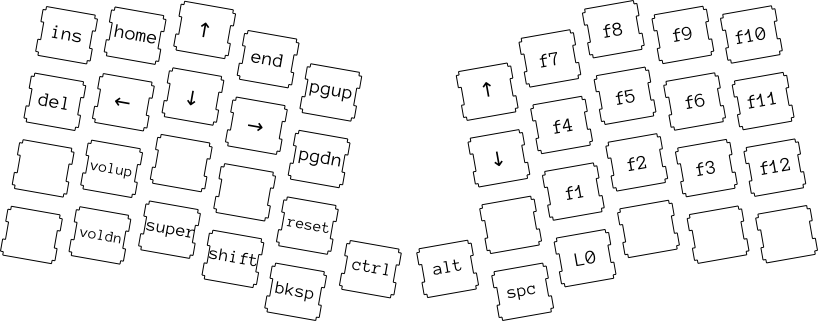
\includegraphics[scale=0.45]{images/atreus-layer-3}
\end{frame}




\begin{frame}
  \frametitle{Open Source}
  Project info:
  \begin{itemize}
    \item Available on Github: github.com/technomancy/atreus
    \item Project site: http://atreus.technomancy.us/
  \end{itemize}
  Containing:
  \begin{itemize}
    \item PCB Files
    \item Laser Cutting Templates
    \item Part List
    \item Firmware
  \end{itemize}
\end{frame}

\begin{frame}
  Thanks!

  - @lorentrogers

  \tiny{(Demo of soldering \& keyboard guts)}
\end{frame}

% Custom firmware
% Why you'd want to change layouts

% How the keys are laid out

% What I discovered about my typing

% Things I'd change
% Extra row outside
% Wider/adjustable split


% The other half of the ecosystem: i3

% The final piece: Vim


\end{document}
